\documentclass[1p]{elsarticle_modified}
%\bibliographystyle{elsarticle-num}

%\usepackage[colorlinks]{hyperref}
%\usepackage{abbrmath_seonhwa} %\Abb, \Ascr, \Acal ,\Abf, \Afrak
\usepackage{amsfonts}
\usepackage{amssymb}
\usepackage{amsmath}
\usepackage{amsthm}
\usepackage{scalefnt}
\usepackage{amsbsy}
\usepackage{kotex}
\usepackage{caption}
\usepackage{subfig}
\usepackage{color}
\usepackage{graphicx}
\usepackage{xcolor} %% white, black, red, green, blue, cyan, magenta, yellow
\usepackage{float}
\usepackage{setspace}
\usepackage{hyperref}

\usepackage{tikz}
\usetikzlibrary{arrows}

\usepackage{multirow}
\usepackage{array} % fixed length table
\usepackage{hhline}

%%%%%%%%%%%%%%%%%%%%%
\makeatletter
\renewcommand*\env@matrix[1][\arraystretch]{%
	\edef\arraystretch{#1}%
	\hskip -\arraycolsep
	\let\@ifnextchar\new@ifnextchar
	\array{*\c@MaxMatrixCols c}}
\makeatother %https://tex.stackexchange.com/questions/14071/how-can-i-increase-the-line-spacing-in-a-matrix
%%%%%%%%%%%%%%%

\usepackage[normalem]{ulem}

\newcommand{\msout}[1]{\ifmmode\text{\sout{\ensuremath{#1}}}\else\sout{#1}\fi}
%SOURCE: \msout is \stkout macro in https://tex.stackexchange.com/questions/20609/strikeout-in-math-mode

\newcommand{\cancel}[1]{
	\ifmmode
	{\color{red}\msout{#1}}
	\else
	{\color{red}\sout{#1}}
	\fi
}

\newcommand{\add}[1]{
	{\color{blue}\uwave{#1}}
}

\newcommand{\replace}[2]{
	\ifmmode
	{\color{red}\msout{#1}}{\color{blue}\uwave{#2}}
	\else
	{\color{red}\sout{#1}}{\color{blue}\uwave{#2}}
	\fi
}

\newcommand{\Sol}{\mathcal{S}} %segment
\newcommand{\D}{D} %diagram
\newcommand{\A}{\mathcal{A}} %arc


%%%%%%%%%%%%%%%%%%%%%%%%%%%%%5 test

\def\sl{\operatorname{\textup{SL}}(2,\Cbb)}
\def\psl{\operatorname{\textup{PSL}}(2,\Cbb)}
\def\quan{\mkern 1mu \triangleright \mkern 1mu}

\theoremstyle{definition}
\newtheorem{thm}{Theorem}[section]
\newtheorem{prop}[thm]{Proposition}
\newtheorem{lem}[thm]{Lemma}
\newtheorem{ques}[thm]{Question}
\newtheorem{cor}[thm]{Corollary}
\newtheorem{defn}[thm]{Definition}
\newtheorem{exam}[thm]{Example}
\newtheorem{rmk}[thm]{Remark}
\newtheorem{alg}[thm]{Algorithm}

\newcommand{\I}{\sqrt{-1}}
\begin{document}

%\begin{frontmatter}
%
%\title{Boundary parabolic representations of knots up to 8 crossings}
%
%%% Group authors per affiliation:
%\author{Yunhi Cho} 
%\address{Department of Mathematics, University of Seoul, Seoul, Korea}
%\ead{yhcho@uos.ac.kr}
%
%
%\author{Seonhwa Kim} %\fnref{s_kim}}
%\address{Center for Geometry and Physics, Institute for Basic Science, Pohang, 37673, Korea}
%\ead{ryeona17@ibs.re.kr}
%
%\author{Hyuk Kim}
%\address{Department of Mathematical Sciences, Seoul National University, Seoul 08826, Korea}
%\ead{hyukkim@snu.ac.kr}
%
%\author{Seokbeom Yoon}
%\address{Department of Mathematical Sciences, Seoul National University, Seoul, 08826,  Korea}
%\ead{sbyoon15@snu.ac.kr}
%
%\begin{abstract}
%We find all boundary parabolic representation of knots up to 8 crossings.
%
%\end{abstract}
%\begin{keyword}
%    \MSC[2010] 57M25 
%\end{keyword}
%
%\end{frontmatter}

%\linenumbers
%\tableofcontents
%
\newcommand\colored[1]{\textcolor{white}{\rule[-0.35ex]{0.8em}{1.4ex}}\kern-0.8em\color{red} #1}%
%\newcommand\colored[1]{\textcolor{white}{ #1}\kern-2.17ex	\textcolor{white}{ #1}\kern-1.81ex	\textcolor{white}{ #1}\kern-2.15ex\color{red}#1	}

{\Large $\underline{12n_{0492}~(K12n_{0492})}$}

\setlength{\tabcolsep}{10pt}
\renewcommand{\arraystretch}{1.6}
\vspace{1cm}\begin{tabular}{m{100pt}>{\centering\arraybackslash}m{274pt}}
\multirow{5}{120pt}{
	\centering
	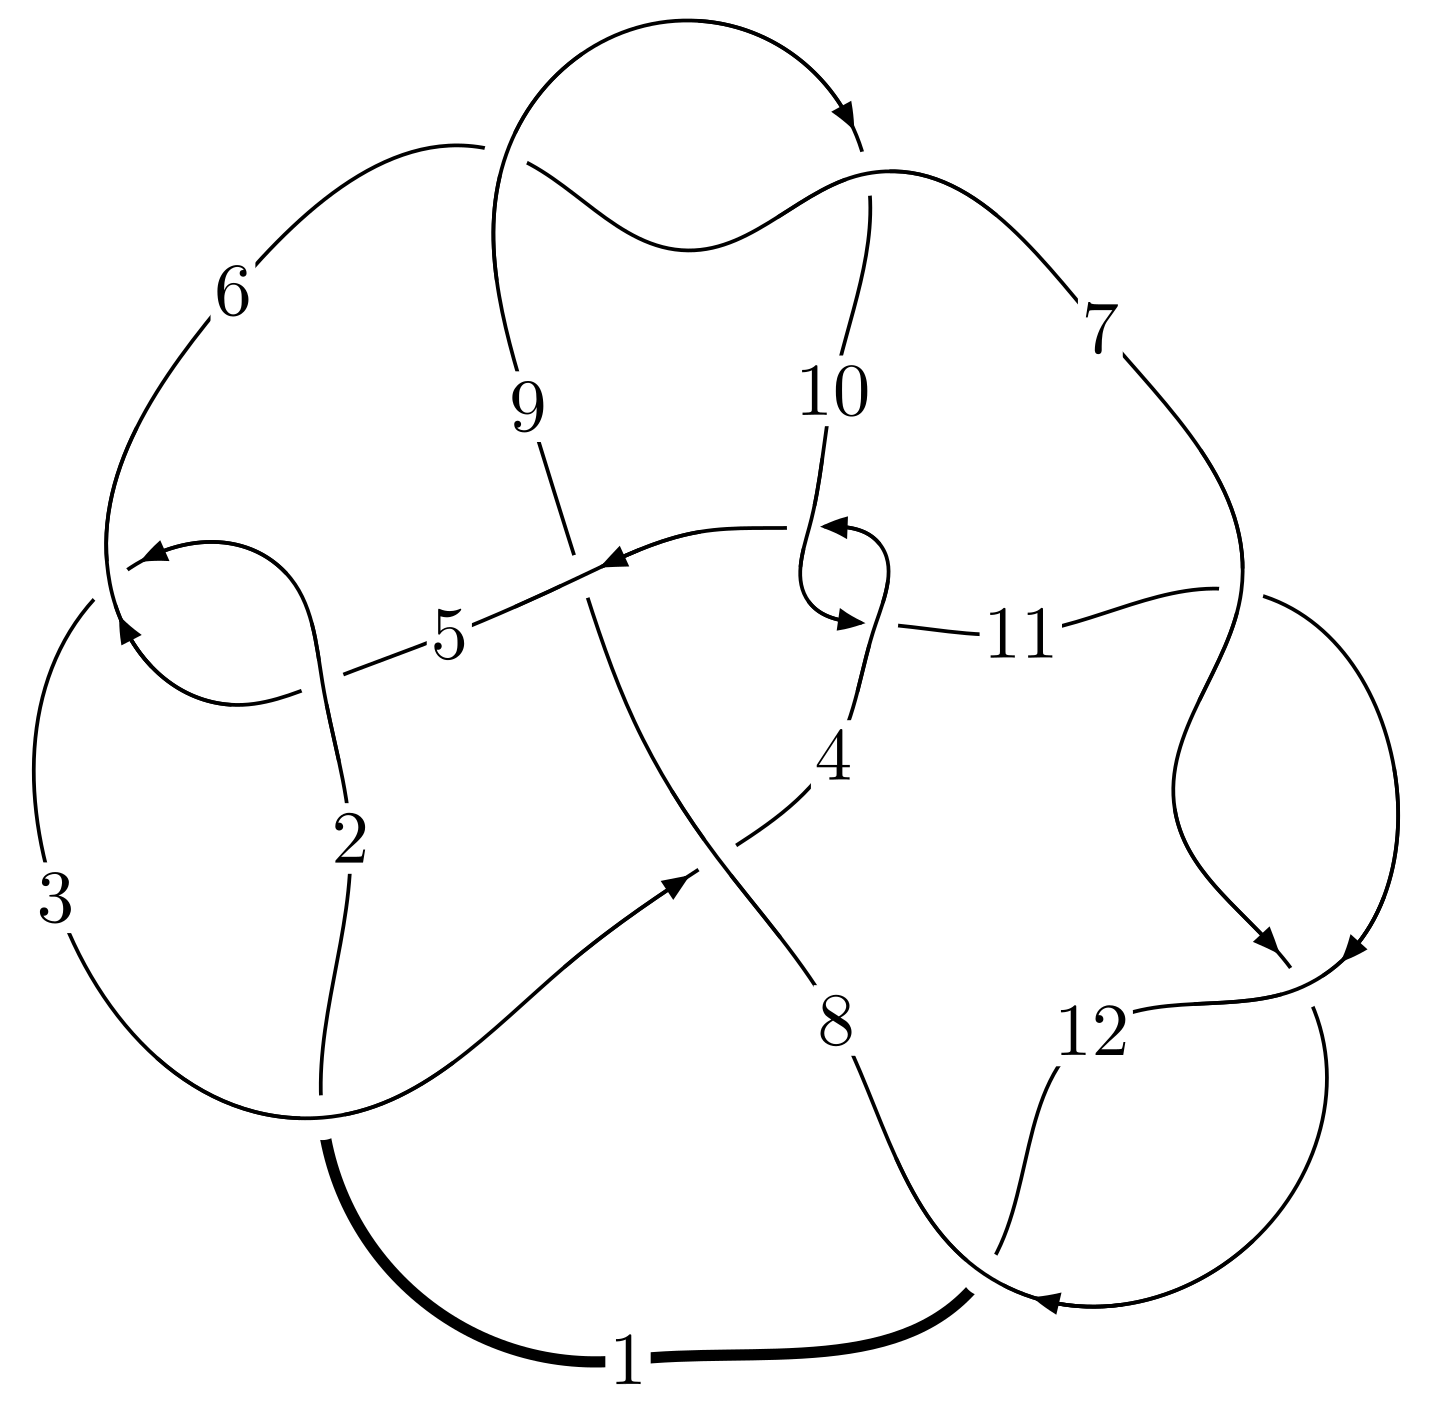
\includegraphics[width=112pt]{../../../GIT/diagram.site/Diagrams/png/2581_12n_0492.png}\\
\ \ \ A knot diagram\footnotemark}&
\allowdisplaybreaks
\textbf{Linearized knot diagam} \\
\cline{2-2}
 &
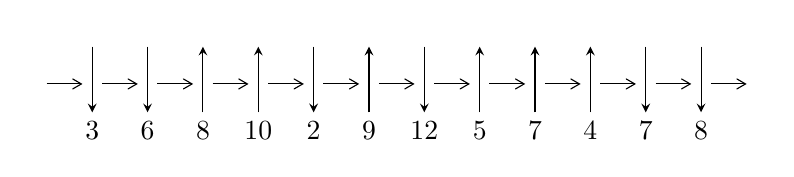
\begin{tikzpicture}[x=20pt, y=17pt]
	% nodes
	\node (C0) at (0, 0) {};
	\node (C1) at (1, 0) {};
	\node (C1U) at (1, +1) {};
	\node (C1D) at (1, -1) {3};

	\node (C2) at (2, 0) {};
	\node (C2U) at (2, +1) {};
	\node (C2D) at (2, -1) {6};

	\node (C3) at (3, 0) {};
	\node (C3U) at (3, +1) {};
	\node (C3D) at (3, -1) {8};

	\node (C4) at (4, 0) {};
	\node (C4U) at (4, +1) {};
	\node (C4D) at (4, -1) {10};

	\node (C5) at (5, 0) {};
	\node (C5U) at (5, +1) {};
	\node (C5D) at (5, -1) {2};

	\node (C6) at (6, 0) {};
	\node (C6U) at (6, +1) {};
	\node (C6D) at (6, -1) {9};

	\node (C7) at (7, 0) {};
	\node (C7U) at (7, +1) {};
	\node (C7D) at (7, -1) {12};

	\node (C8) at (8, 0) {};
	\node (C8U) at (8, +1) {};
	\node (C8D) at (8, -1) {5};

	\node (C9) at (9, 0) {};
	\node (C9U) at (9, +1) {};
	\node (C9D) at (9, -1) {7};

	\node (C10) at (10, 0) {};
	\node (C10U) at (10, +1) {};
	\node (C10D) at (10, -1) {4};

	\node (C11) at (11, 0) {};
	\node (C11U) at (11, +1) {};
	\node (C11D) at (11, -1) {7};

	\node (C12) at (12, 0) {};
	\node (C12U) at (12, +1) {};
	\node (C12D) at (12, -1) {8};
	\node (C13) at (13, 0) {};

	% arrows
	\draw[->,>={angle 60}]
	(C0) edge (C1) (C1) edge (C2) (C2) edge (C3) (C3) edge (C4) (C4) edge (C5) (C5) edge (C6) (C6) edge (C7) (C7) edge (C8) (C8) edge (C9) (C9) edge (C10) (C10) edge (C11) (C11) edge (C12) (C12) edge (C13) ;	\draw[->,>=stealth]
	(C1U) edge (C1D) (C2U) edge (C2D) (C3D) edge (C3U) (C4D) edge (C4U) (C5U) edge (C5D) (C6D) edge (C6U) (C7U) edge (C7D) (C8D) edge (C8U) (C9D) edge (C9U) (C10D) edge (C10U) (C11U) edge (C11D) (C12U) edge (C12D) ;
	\end{tikzpicture} \\
\hhline{~~} \\& 
\textbf{Solving Sequence} \\ \cline{2-2} 
 &
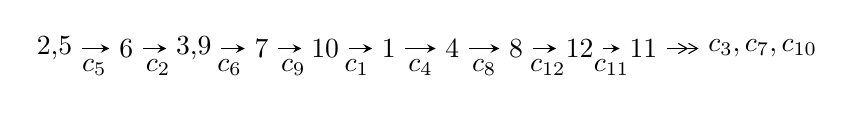
\begin{tikzpicture}[x=23pt, y=7pt]
	% node
	\node (A0) at (-1/8, 0) {2,5};
	\node (A1) at (1, 0) {6};
	\node (A2) at (33/16, 0) {3,9};
	\node (A3) at (25/8, 0) {7};
	\node (A4) at (33/8, 0) {10};
	\node (A5) at (41/8, 0) {1};
	\node (A6) at (49/8, 0) {4};
	\node (A7) at (57/8, 0) {8};
	\node (A8) at (65/8, 0) {12};
	\node (A9) at (73/8, 0) {11};
	\node (C1) at (1/2, -1) {$c_{5}$};
	\node (C2) at (3/2, -1) {$c_{2}$};
	\node (C3) at (21/8, -1) {$c_{6}$};
	\node (C4) at (29/8, -1) {$c_{9}$};
	\node (C5) at (37/8, -1) {$c_{1}$};
	\node (C6) at (45/8, -1) {$c_{4}$};
	\node (C7) at (53/8, -1) {$c_{8}$};
	\node (C8) at (61/8, -1) {$c_{12}$};
	\node (C9) at (69/8, -1) {$c_{11}$};
	\node (A10) at (11, 0) {$c_{3},c_{7},c_{10}$};

	% edge
	\draw[->,>=stealth]	
	(A0) edge (A1) (A1) edge (A2) (A2) edge (A3) (A3) edge (A4) (A4) edge (A5) (A5) edge (A6) (A6) edge (A7) (A7) edge (A8) (A8) edge (A9) ;
	\draw[->>,>={angle 60}]	
	(A9) edge (A10);
\end{tikzpicture} \\ 

\end{tabular} \\

\footnotetext{
The image of knot diagram is generated by the software ``\textbf{Draw programme}" developed by Andrew Bartholomew(\url{http://www.layer8.co.uk/maths/draw/index.htm\#Running-draw}), where we modified some parts for our purpose(\url{https://github.com/CATsTAILs/LinksPainter}).
}\phantom \\ \newline 
\centering \textbf{Ideals for irreducible components\footnotemark of $X_{\text{par}}$} 
 
\begin{align*}
I^u_{1}&=\langle 
4.46973\times10^{50} u^{60}+8.99199\times10^{50} u^{59}+\cdots+8.26421\times10^{50} b-5.17817\times10^{50},\\
\phantom{I^u_{1}}&\phantom{= \langle  }3.56747\times10^{51} u^{60}+4.54307\times10^{51} u^{59}+\cdots+1.57020\times10^{52} a-1.57657\times10^{52},\;u^{61}+2 u^{60}+\cdots+17 u+19\rangle \\
I^u_{2}&=\langle 
u^{15}+u^{14}-2 u^{13}-2 u^{12}+6 u^{11}+6 u^{10}-8 u^9-6 u^8+11 u^7+9 u^6-9 u^5-5 u^4+6 u^3+3 u^2+b-2 u-1,\\
\phantom{I^u_{2}}&\phantom{= \langle  }u^{14}+2 u^{13}- u^{12}-3 u^{11}+4 u^{10}+8 u^9-3 u^8-5 u^7+7 u^6+5 u^5-3 u^4+3 u^2+a- u,\;u^{17}+u^{16}+\cdots+u+1\rangle \\
\\
\end{align*}
\raggedright * 2 irreducible components of $\dim_{\mathbb{C}}=0$, with total 78 representations.\\
\footnotetext{All coefficients of polynomials are rational numbers. But the coefficients are sometimes approximated in decimal forms when there is not enough margin.}
\newpage
\renewcommand{\arraystretch}{1}
\centering \section*{I. $I^u_{1}= \langle 4.47\times10^{50} u^{60}+8.99\times10^{50} u^{59}+\cdots+8.26\times10^{50} b-5.18\times10^{50},\;3.57\times10^{51} u^{60}+4.54\times10^{51} u^{59}+\cdots+1.57\times10^{52} a-1.58\times10^{52},\;u^{61}+2 u^{60}+\cdots+17 u+19 \rangle$}
\flushleft \textbf{(i) Arc colorings}\\
\begin{tabular}{m{7pt} m{180pt} m{7pt} m{180pt} }
\flushright $a_{2}=$&$\begin{pmatrix}0\\u\end{pmatrix}$ \\
\flushright $a_{5}=$&$\begin{pmatrix}1\\0\end{pmatrix}$ \\
\flushright $a_{6}=$&$\begin{pmatrix}1\\u^2\end{pmatrix}$ \\
\flushright $a_{3}=$&$\begin{pmatrix}- u\\- u^3+u\end{pmatrix}$ \\
\flushright $a_{9}=$&$\begin{pmatrix}-0.227198 u^{60}-0.289331 u^{59}+\cdots-26.0080 u+1.00406\\-0.540853 u^{60}-1.08806 u^{59}+\cdots+4.86169 u+0.626578\end{pmatrix}$ \\
\flushright $a_{7}=$&$\begin{pmatrix}0.253819 u^{60}+0.465067 u^{59}+\cdots-3.89004 u+7.64807\\0.300175 u^{60}+0.771180 u^{59}+\cdots-12.1668 u-2.42640\end{pmatrix}$ \\
\flushright $a_{10}=$&$\begin{pmatrix}0.676302 u^{60}+0.841602 u^{59}+\cdots+3.47497 u+9.49090\\0.207184 u^{60}+0.269966 u^{59}+\cdots-4.37631 u-0.968624\end{pmatrix}$ \\
\flushright $a_{1}=$&$\begin{pmatrix}u^3\\u^5- u^3+u\end{pmatrix}$ \\
\flushright $a_{4}=$&$\begin{pmatrix}-0.274794 u^{60}-0.333191 u^{59}+\cdots-3.80176 u-15.2300\\-0.503752 u^{60}-0.859618 u^{59}+\cdots+9.74194 u-3.86368\end{pmatrix}$ \\
\flushright $a_{8}=$&$\begin{pmatrix}0.313655 u^{60}+0.798733 u^{59}+\cdots-30.8697 u+0.377479\\-0.540853 u^{60}-1.08806 u^{59}+\cdots+4.86169 u+0.626578\end{pmatrix}$ \\
\flushright $a_{12}=$&$\begin{pmatrix}-0.459255 u^{60}-0.619696 u^{59}+\cdots+4.13848 u-10.2887\\0.255017 u^{60}+0.385918 u^{59}+\cdots-11.3938 u-6.86607\end{pmatrix}$ \\
\flushright $a_{11}=$&$\begin{pmatrix}-1.18571 u^{60}-1.47546 u^{59}+\cdots-4.66063 u-37.2565\\-0.0486439 u^{60}-0.362172 u^{59}+\cdots+2.29122 u-3.22234\end{pmatrix}$\\&\end{tabular}
\flushleft \textbf{(ii) Obstruction class $= -1$}\\~\\
\flushleft \textbf{(iii) Cusp Shapes $= -0.599933 u^{60}-0.940036 u^{59}+\cdots-28.5387 u+5.37229$}\\~\\
\newpage\renewcommand{\arraystretch}{1}
\flushleft \textbf{(iv) u-Polynomials at the component}\newline \\
\begin{tabular}{m{50pt}|m{274pt}}
Crossings & \hspace{64pt}u-Polynomials at each crossing \\
\hline $$\begin{aligned}c_{1}\end{aligned}$$&$\begin{aligned}
&u^{61}+18 u^{60}+\cdots+5229 u+361
\end{aligned}$\\
\hline $$\begin{aligned}c_{2},c_{5}\end{aligned}$$&$\begin{aligned}
&u^{61}+2 u^{60}+\cdots+17 u+19
\end{aligned}$\\
\hline $$\begin{aligned}c_{3}\end{aligned}$$&$\begin{aligned}
&u^{61}+2 u^{60}+\cdots+82113 u+15047
\end{aligned}$\\
\hline $$\begin{aligned}c_{4},c_{10}\end{aligned}$$&$\begin{aligned}
&u^{61}+3 u^{60}+\cdots+21 u+1
\end{aligned}$\\
\hline $$\begin{aligned}c_{6},c_{9}\end{aligned}$$&$\begin{aligned}
&u^{61}-28 u^{59}+\cdots-4 u+1
\end{aligned}$\\
\hline $$\begin{aligned}c_{7},c_{11},c_{12}\end{aligned}$$&$\begin{aligned}
&u^{61}+u^{60}+\cdots+15 u-1
\end{aligned}$\\
\hline $$\begin{aligned}c_{8}\end{aligned}$$&$\begin{aligned}
&u^{61}- u^{60}+\cdots+5 u-11
\end{aligned}$\\
\hline
\end{tabular}\\~\\
\newpage\renewcommand{\arraystretch}{1}
\flushleft \textbf{(v) Riley Polynomials at the component}\newline \\
\begin{tabular}{m{50pt}|m{274pt}}
Crossings & \hspace{64pt}Riley Polynomials at each crossing \\
\hline $$\begin{aligned}c_{1}\end{aligned}$$&$\begin{aligned}
&y^{61}+58 y^{60}+\cdots-1648747 y-130321
\end{aligned}$\\
\hline $$\begin{aligned}c_{2},c_{5}\end{aligned}$$&$\begin{aligned}
&y^{61}-18 y^{60}+\cdots+5229 y-361
\end{aligned}$\\
\hline $$\begin{aligned}c_{3}\end{aligned}$$&$\begin{aligned}
&y^{61}-72 y^{60}+\cdots+15660841481 y-226412209
\end{aligned}$\\
\hline $$\begin{aligned}c_{4},c_{10}\end{aligned}$$&$\begin{aligned}
&y^{61}+17 y^{60}+\cdots+63 y-1
\end{aligned}$\\
\hline $$\begin{aligned}c_{6},c_{9}\end{aligned}$$&$\begin{aligned}
&y^{61}-56 y^{60}+\cdots+94 y-1
\end{aligned}$\\
\hline $$\begin{aligned}c_{7},c_{11},c_{12}\end{aligned}$$&$\begin{aligned}
&y^{61}-15 y^{60}+\cdots+31 y-1
\end{aligned}$\\
\hline $$\begin{aligned}c_{8}\end{aligned}$$&$\begin{aligned}
&y^{61}+y^{60}+\cdots+7945 y-121
\end{aligned}$\\
\hline
\end{tabular}\\~\\
\newpage\flushleft \textbf{(vi) Complex Volumes and Cusp Shapes}
$$\begin{array}{c|c|c}  
\text{Solutions to }I^u_{1}& \I (\text{vol} + \sqrt{-1}CS) & \text{Cusp shape}\\
 \hline 
\begin{aligned}
u &= \phantom{-}1.008560 + 0.099272 I \\
a &= -0.30905 - 1.85898 I \\
b &= \phantom{-}0.359420 - 0.718984 I\end{aligned}
 & -3.62853 - 2.81695 I & -7.75571 + 7.59659 I \\ \hline\begin{aligned}
u &= \phantom{-}1.008560 - 0.099272 I \\
a &= -0.30905 + 1.85898 I \\
b &= \phantom{-}0.359420 + 0.718984 I\end{aligned}
 & -3.62853 + 2.81695 I & -7.75571 - 7.59659 I \\ \hline\begin{aligned}
u &= \phantom{-}0.059768 + 1.029870 I \\
a &= \phantom{-}0.357240 + 0.027030 I \\
b &= \phantom{-}0.775249 + 0.356076 I\end{aligned}
 & \phantom{-}3.37069 + 4.37380 I & \phantom{-}4.08170 - 9.15688 I \\ \hline\begin{aligned}
u &= \phantom{-}0.059768 - 1.029870 I \\
a &= \phantom{-}0.357240 - 0.027030 I \\
b &= \phantom{-}0.775249 - 0.356076 I\end{aligned}
 & \phantom{-}3.37069 - 4.37380 I & \phantom{-}4.08170 + 9.15688 I \\ \hline\begin{aligned}
u &= -0.711308 + 0.756370 I \\
a &= \phantom{-}0.898738 + 0.163809 I \\
b &= -0.502080 + 0.422908 I\end{aligned}
 & \phantom{-}2.16071 - 2.54963 I & -1.92850 + 5.48932 I \\ \hline\begin{aligned}
u &= -0.711308 - 0.756370 I \\
a &= \phantom{-}0.898738 - 0.163809 I \\
b &= -0.502080 - 0.422908 I\end{aligned}
 & \phantom{-}2.16071 + 2.54963 I & -1.92850 - 5.48932 I \\ \hline\begin{aligned}
u &= -0.802317 + 0.516125 I \\
a &= -1.53275 + 0.59230 I \\
b &= \phantom{-}0.14998 + 1.42541 I\end{aligned}
 & -6.39239 + 2.05870 I & -6.76486 - 3.26008 I \\ \hline\begin{aligned}
u &= -0.802317 - 0.516125 I \\
a &= -1.53275 - 0.59230 I \\
b &= \phantom{-}0.14998 - 1.42541 I\end{aligned}
 & -6.39239 - 2.05870 I & -6.76486 + 3.26008 I \\ \hline\begin{aligned}
u &= \phantom{-}0.681279 + 0.639801 I \\
a &= \phantom{-}0.355489 - 0.164381 I \\
b &= -1.136570 - 0.305208 I\end{aligned}
 & \phantom{-}2.72340 + 1.00029 I & -0.33756 + 1.68143 I \\ \hline\begin{aligned}
u &= \phantom{-}0.681279 - 0.639801 I \\
a &= \phantom{-}0.355489 + 0.164381 I \\
b &= -1.136570 + 0.305208 I\end{aligned}
 & \phantom{-}2.72340 - 1.00029 I & -0.33756 - 1.68143 I\\
 \hline 
 \end{array}$$\newpage$$\begin{array}{c|c|c}  
\text{Solutions to }I^u_{1}& \I (\text{vol} + \sqrt{-1}CS) & \text{Cusp shape}\\
 \hline 
\begin{aligned}
u &= -0.855118 + 0.666348 I \\
a &= \phantom{-}0.79912 - 1.53720 I \\
b &= \phantom{-}0.044913 - 1.261780 I\end{aligned}
 & -1.78842 + 2.57888 I & \phantom{-}3.59230 - 3.67922 I \\ \hline\begin{aligned}
u &= -0.855118 - 0.666348 I \\
a &= \phantom{-}0.79912 + 1.53720 I \\
b &= \phantom{-}0.044913 + 1.261780 I\end{aligned}
 & -1.78842 - 2.57888 I & \phantom{-}3.59230 + 3.67922 I \\ \hline\begin{aligned}
u &= -0.830799 + 0.768291 I \\
a &= \phantom{-}0.040905 - 0.410536 I \\
b &= \phantom{-}0.438873 - 0.240508 I\end{aligned}
 & -0.20731 + 2.69693 I & -1.60164 - 3.85142 I \\ \hline\begin{aligned}
u &= -0.830799 - 0.768291 I \\
a &= \phantom{-}0.040905 + 0.410536 I \\
b &= \phantom{-}0.438873 + 0.240508 I\end{aligned}
 & -0.20731 - 2.69693 I & -1.60164 + 3.85142 I \\ \hline\begin{aligned}
u &= -1.132350 + 0.015313 I \\
a &= \phantom{-}0.529981 - 0.317231 I \\
b &= \phantom{-}0.499234 - 0.170729 I\end{aligned}
 & -2.57618 + 0.03241 I & -6.83473 + 2.23858 I \\ \hline\begin{aligned}
u &= -1.132350 - 0.015313 I \\
a &= \phantom{-}0.529981 + 0.317231 I \\
b &= \phantom{-}0.499234 + 0.170729 I\end{aligned}
 & -2.57618 - 0.03241 I & -6.83473 - 2.23858 I \\ \hline\begin{aligned}
u &= \phantom{-}0.797110 + 0.332880 I \\
a &= \phantom{-}0.93154 - 2.92490 I \\
b &= \phantom{-}0.573126 - 0.489509 I\end{aligned}
 & \phantom{-}1.86824 - 4.30118 I & -1.43694 + 7.83913 I \\ \hline\begin{aligned}
u &= \phantom{-}0.797110 - 0.332880 I \\
a &= \phantom{-}0.93154 + 2.92490 I \\
b &= \phantom{-}0.573126 + 0.489509 I\end{aligned}
 & \phantom{-}1.86824 + 4.30118 I & -1.43694 - 7.83913 I \\ \hline\begin{aligned}
u &= -1.005330 + 0.593094 I \\
a &= \phantom{-}0.285708 - 1.177370 I \\
b &= -0.222145 - 0.767554 I\end{aligned}
 & -0.86882 + 2.72261 I & -4.26405 + 0. I\phantom{ +0.000000I} \\ \hline\begin{aligned}
u &= -1.005330 - 0.593094 I \\
a &= \phantom{-}0.285708 + 1.177370 I \\
b &= -0.222145 + 0.767554 I\end{aligned}
 & -0.86882 - 2.72261 I & -4.26405 + 0. I\phantom{ +0.000000I}\\
 \hline 
 \end{array}$$\newpage$$\begin{array}{c|c|c}  
\text{Solutions to }I^u_{1}& \I (\text{vol} + \sqrt{-1}CS) & \text{Cusp shape}\\
 \hline 
\begin{aligned}
u &= \phantom{-}0.778504 + 0.873488 I \\
a &= \phantom{-}0.212728 + 0.508358 I \\
b &= -0.949362 + 0.147769 I\end{aligned}
 & \phantom{-}4.30301 - 0.06144 I & \phantom{-}4.49581 + 0. I\phantom{ +0.000000I} \\ \hline\begin{aligned}
u &= \phantom{-}0.778504 - 0.873488 I \\
a &= \phantom{-}0.212728 - 0.508358 I \\
b &= -0.949362 - 0.147769 I\end{aligned}
 & \phantom{-}4.30301 + 0.06144 I & \phantom{-}4.49581 + 0. I\phantom{ +0.000000I} \\ \hline\begin{aligned}
u &= -0.760268 + 0.241047 I \\
a &= -0.398024 + 1.076770 I \\
b &= -1.232000 + 0.398283 I\end{aligned}
 & \phantom{-}1.36337 + 3.68980 I & -4.58791 - 6.16767 I \\ \hline\begin{aligned}
u &= -0.760268 - 0.241047 I \\
a &= -0.398024 - 1.076770 I \\
b &= -1.232000 - 0.398283 I\end{aligned}
 & \phantom{-}1.36337 - 3.68980 I & -4.58791 + 6.16767 I \\ \hline\begin{aligned}
u &= \phantom{-}0.876318 + 0.829854 I \\
a &= -0.77583 - 1.74978 I \\
b &= \phantom{-}1.21040 - 1.31023 I\end{aligned}
 & \phantom{-}7.73388 + 0.14159 I & \phantom{-0.000000 } 0 \\ \hline\begin{aligned}
u &= \phantom{-}0.876318 - 0.829854 I \\
a &= -0.77583 + 1.74978 I \\
b &= \phantom{-}1.21040 + 1.31023 I\end{aligned}
 & \phantom{-}7.73388 - 0.14159 I & \phantom{-0.000000 } 0 \\ \hline\begin{aligned}
u &= \phantom{-}1.001920 + 0.674098 I \\
a &= -0.35058 - 1.68445 I \\
b &= \phantom{-}1.048960 - 0.498864 I\end{aligned}
 & \phantom{-}1.72001 - 6.24237 I & \phantom{-0.000000 } 0 \\ \hline\begin{aligned}
u &= \phantom{-}1.001920 - 0.674098 I \\
a &= -0.35058 + 1.68445 I \\
b &= \phantom{-}1.048960 + 0.498864 I\end{aligned}
 & \phantom{-}1.72001 + 6.24237 I & \phantom{-0.000000 } 0 \\ \hline\begin{aligned}
u &= -0.859996 + 0.852993 I \\
a &= -0.505439 + 0.295038 I \\
b &= -1.21247 + 1.10581 I\end{aligned}
 & \phantom{-}9.10418 - 0.98120 I & \phantom{-0.000000 } 0 \\ \hline\begin{aligned}
u &= -0.859996 - 0.852993 I \\
a &= -0.505439 - 0.295038 I \\
b &= -1.21247 - 1.10581 I\end{aligned}
 & \phantom{-}9.10418 + 0.98120 I & \phantom{-0.000000 } 0\\
 \hline 
 \end{array}$$\newpage$$\begin{array}{c|c|c}  
\text{Solutions to }I^u_{1}& \I (\text{vol} + \sqrt{-1}CS) & \text{Cusp shape}\\
 \hline 
\begin{aligned}
u &= \phantom{-}0.743198 + 0.258578 I \\
a &= \phantom{-}1.14961 + 2.70783 I \\
b &= -0.02378 + 1.65985 I\end{aligned}
 & -7.66046 - 1.07355 I & -0.63774 + 8.35173 I \\ \hline\begin{aligned}
u &= \phantom{-}0.743198 - 0.258578 I \\
a &= \phantom{-}1.14961 - 2.70783 I \\
b &= -0.02378 - 1.65985 I\end{aligned}
 & -7.66046 + 1.07355 I & -0.63774 - 8.35173 I \\ \hline\begin{aligned}
u &= -0.985859 + 0.708002 I \\
a &= -1.18958 + 1.16281 I \\
b &= \phantom{-}0.603722 + 0.517705 I\end{aligned}
 & \phantom{-}1.33700 + 8.12439 I & \phantom{-0.000000 } 0. - 11.41912 I \\ \hline\begin{aligned}
u &= -0.985859 - 0.708002 I \\
a &= -1.18958 - 1.16281 I \\
b &= \phantom{-}0.603722 - 0.517705 I\end{aligned}
 & \phantom{-}1.33700 - 8.12439 I & \phantom{-0.000000 -}0. + 11.41912 I \\ \hline\begin{aligned}
u &= -0.747298 + 0.958094 I \\
a &= \phantom{-}0.384523 - 0.093109 I \\
b &= \phantom{-}1.27040 - 1.04462 I\end{aligned}
 & \phantom{-}8.45288 - 9.12237 I & \phantom{-0.000000 } 0 \\ \hline\begin{aligned}
u &= -0.747298 - 0.958094 I \\
a &= \phantom{-}0.384523 + 0.093109 I \\
b &= \phantom{-}1.27040 + 1.04462 I\end{aligned}
 & \phantom{-}8.45288 + 9.12237 I & \phantom{-0.000000 } 0 \\ \hline\begin{aligned}
u &= \phantom{-}0.513333 + 0.577329 I \\
a &= \phantom{-}0.147645 - 0.303415 I \\
b &= -1.097740 - 0.294525 I\end{aligned}
 & \phantom{-}2.71819 + 1.05648 I & \phantom{-}1.23406 + 1.60799 I \\ \hline\begin{aligned}
u &= \phantom{-}0.513333 - 0.577329 I \\
a &= \phantom{-}0.147645 + 0.303415 I \\
b &= -1.097740 + 0.294525 I\end{aligned}
 & \phantom{-}2.71819 - 1.05648 I & \phantom{-}1.23406 - 1.60799 I \\ \hline\begin{aligned}
u &= \phantom{-}0.920582 + 0.813292 I \\
a &= -0.834573 - 0.068760 I \\
b &= -1.38008 - 1.21627 I\end{aligned}
 & \phantom{-}7.59405 - 6.27627 I & \phantom{-0.000000 } 0 \\ \hline\begin{aligned}
u &= \phantom{-}0.920582 - 0.813292 I \\
a &= -0.834573 + 0.068760 I \\
b &= -1.38008 + 1.21627 I\end{aligned}
 & \phantom{-}7.59405 + 6.27627 I & \phantom{-0.000000 } 0\\
 \hline 
 \end{array}$$\newpage$$\begin{array}{c|c|c}  
\text{Solutions to }I^u_{1}& \I (\text{vol} + \sqrt{-1}CS) & \text{Cusp shape}\\
 \hline 
\begin{aligned}
u &= \phantom{-}1.188700 + 0.367540 I \\
a &= -0.51935 + 1.50281 I \\
b &= -0.734725 + 0.839423 I\end{aligned}
 & -0.58425 - 9.12112 I & \phantom{-0.000000 } 0 \\ \hline\begin{aligned}
u &= \phantom{-}1.188700 - 0.367540 I \\
a &= -0.51935 - 1.50281 I \\
b &= -0.734725 - 0.839423 I\end{aligned}
 & -0.58425 + 9.12112 I & \phantom{-0.000000 } 0 \\ \hline\begin{aligned}
u &= -0.943245 + 0.820348 I \\
a &= -0.77128 + 1.86248 I \\
b &= \phantom{-}1.05879 + 1.19926 I\end{aligned}
 & \phantom{-}8.84141 + 7.20713 I & \phantom{-0.000000 } 0 \\ \hline\begin{aligned}
u &= -0.943245 - 0.820348 I \\
a &= -0.77128 - 1.86248 I \\
b &= \phantom{-}1.05879 - 1.19926 I\end{aligned}
 & \phantom{-}8.84141 - 7.20713 I & \phantom{-0.000000 } 0 \\ \hline\begin{aligned}
u &= \phantom{-}0.816581 + 0.959000 I \\
a &= \phantom{-}0.543543 + 0.025883 I \\
b &= \phantom{-}1.20038 + 0.96984 I\end{aligned}
 & \phantom{-}9.60140 + 1.01873 I & \phantom{-0.000000 } 0 \\ \hline\begin{aligned}
u &= \phantom{-}0.816581 - 0.959000 I \\
a &= \phantom{-}0.543543 - 0.025883 I \\
b &= \phantom{-}1.20038 - 0.96984 I\end{aligned}
 & \phantom{-}9.60140 - 1.01873 I & \phantom{-0.000000 } 0 \\ \hline\begin{aligned}
u &= \phantom{-}0.729689 + 0.092257 I \\
a &= -2.17992 - 1.30658 I \\
b &= \phantom{-}0.296181 - 0.865356 I\end{aligned}
 & -4.76315 - 0.37609 I & -6.92192 - 3.20821 I \\ \hline\begin{aligned}
u &= \phantom{-}0.729689 - 0.092257 I \\
a &= -2.17992 + 1.30658 I \\
b &= \phantom{-}0.296181 + 0.865356 I\end{aligned}
 & -4.76315 + 0.37609 I & -6.92192 + 3.20821 I \\ \hline\begin{aligned}
u &= -0.958783 + 0.851896 I \\
a &= \phantom{-}0.574031 - 0.735538 I \\
b &= -0.272425 - 0.985135 I\end{aligned}
 & -0.94086 + 3.29997 I & \phantom{-0.000000 } 0 \\ \hline\begin{aligned}
u &= -0.958783 - 0.851896 I \\
a &= \phantom{-}0.574031 + 0.735538 I \\
b &= -0.272425 + 0.985135 I\end{aligned}
 & -0.94086 - 3.29997 I & \phantom{-0.000000 } 0\\
 \hline 
 \end{array}$$\newpage$$\begin{array}{c|c|c}  
\text{Solutions to }I^u_{1}& \I (\text{vol} + \sqrt{-1}CS) & \text{Cusp shape}\\
 \hline 
\begin{aligned}
u &= \phantom{-}1.008090 + 0.801211 I \\
a &= \phantom{-}0.049974 - 0.714510 I \\
b &= \phantom{-}1.004090 - 0.082477 I\end{aligned}
 & \phantom{-}3.59655 - 6.16597 I & \phantom{-0.000000 } 0 \\ \hline\begin{aligned}
u &= \phantom{-}1.008090 - 0.801211 I \\
a &= \phantom{-}0.049974 + 0.714510 I \\
b &= \phantom{-}1.004090 + 0.082477 I\end{aligned}
 & \phantom{-}3.59655 + 6.16597 I & \phantom{-0.000000 } 0 \\ \hline\begin{aligned}
u &= -0.634593 + 0.305711 I \\
a &= \phantom{-}1.70511 + 2.78485 I \\
b &= \phantom{-}0.475869 + 0.583891 I\end{aligned}
 & \phantom{-}1.76589 - 1.46394 I & -2.18428 - 1.39749 I \\ \hline\begin{aligned}
u &= -0.634593 - 0.305711 I \\
a &= \phantom{-}1.70511 - 2.78485 I \\
b &= \phantom{-}0.475869 - 0.583891 I\end{aligned}
 & \phantom{-}1.76589 + 1.46394 I & -2.18428 + 1.39749 I \\ \hline\begin{aligned}
u &= -1.32936\phantom{ +0.000000I} \\
a &= -0.425742\phantom{ +0.000000I} \\
b &= -0.130836\phantom{ +0.000000I}\end{aligned}
 & -2.35229\phantom{ +0.000000I} & \phantom{-0.000000 } 0 \\ \hline\begin{aligned}
u &= \phantom{-}1.022890 + 0.850141 I \\
a &= \phantom{-}0.46632 + 1.56053 I \\
b &= -1.17031 + 1.15196 I\end{aligned}
 & \phantom{-}8.93314 - 7.65090 I & \phantom{-0.000000 } 0 \\ \hline\begin{aligned}
u &= \phantom{-}1.022890 - 0.850141 I \\
a &= \phantom{-}0.46632 - 1.56053 I \\
b &= -1.17031 - 1.15196 I\end{aligned}
 & \phantom{-}8.93314 + 7.65090 I & \phantom{-0.000000 } 0 \\ \hline\begin{aligned}
u &= -1.054050 + 0.811352 I \\
a &= \phantom{-}0.55964 - 1.79633 I \\
b &= -1.23639 - 1.18766 I\end{aligned}
 & \phantom{-}7.4752 + 15.6144 I & \phantom{-0.000000 } 0 \\ \hline\begin{aligned}
u &= -1.054050 - 0.811352 I \\
a &= \phantom{-}0.55964 + 1.79633 I \\
b &= -1.23639 + 1.18766 I\end{aligned}
 & \phantom{-}7.4752 - 15.6144 I & \phantom{-0.000000 } 0 \\ \hline\begin{aligned}
u &= -0.200523 + 0.477929 I \\
a &= \phantom{-}0.745281 - 0.474801 I \\
b &= -0.274077 - 0.499104 I\end{aligned}
 & \phantom{-}0.075701 + 1.180500 I & \phantom{-}0.98721 - 5.73205 I\\
 \hline 
 \end{array}$$\newpage$$\begin{array}{c|c|c}  
\text{Solutions to }I^u_{1}& \I (\text{vol} + \sqrt{-1}CS) & \text{Cusp shape}\\
 \hline 
\begin{aligned}
u &= -0.200523 - 0.477929 I \\
a &= \phantom{-}0.745281 + 0.474801 I \\
b &= -0.274077 + 0.499104 I\end{aligned}
 & \phantom{-}0.075701 - 1.180500 I & \phantom{-}0.98721 + 5.73205 I\\
 \hline 
 \end{array}$$\newpage\newpage\renewcommand{\arraystretch}{1}
\centering \section*{II. $I^u_{2}= \langle u^{15}+u^{14}+\cdots+b-1,\;u^{14}+2 u^{13}+\cdots+a- u,\;u^{17}+u^{16}+\cdots+u+1 \rangle$}
\flushleft \textbf{(i) Arc colorings}\\
\begin{tabular}{m{7pt} m{180pt} m{7pt} m{180pt} }
\flushright $a_{2}=$&$\begin{pmatrix}0\\u\end{pmatrix}$ \\
\flushright $a_{5}=$&$\begin{pmatrix}1\\0\end{pmatrix}$ \\
\flushright $a_{6}=$&$\begin{pmatrix}1\\u^2\end{pmatrix}$ \\
\flushright $a_{3}=$&$\begin{pmatrix}- u\\- u^3+u\end{pmatrix}$ \\
\flushright $a_{9}=$&$\begin{pmatrix}- u^{14}-2 u^{13}+\cdots-3 u^2+u\\- u^{15}- u^{14}+\cdots+2 u+1\end{pmatrix}$ \\
\flushright $a_{7}=$&$\begin{pmatrix}2 u^{16}+u^{15}+\cdots-11 u^2+3\\u^{13}+u^{12}+\cdots- u^2+u\end{pmatrix}$ \\
\flushright $a_{10}=$&$\begin{pmatrix}-2 u^{16}-2 u^{15}+\cdots+u+1\\- u^{16}- u^{15}+\cdots-2 u^2+1\end{pmatrix}$ \\
\flushright $a_{1}=$&$\begin{pmatrix}u^3\\u^5- u^3+u\end{pmatrix}$ \\
\flushright $a_{4}=$&$\begin{pmatrix}u^{16}+3 u^{15}+\cdots-6 u-2\\u^{16}+u^{15}+\cdots-5 u^2-2 u\end{pmatrix}$ \\
\flushright $a_{8}=$&$\begin{pmatrix}u^{15}-4 u^{13}+\cdots- u-1\\- u^{15}- u^{14}+\cdots+2 u+1\end{pmatrix}$ \\
\flushright $a_{12}=$&$\begin{pmatrix}- u^{16}+u^{15}+\cdots+8 u^2-2\\2 u^{16}+2 u^{15}+\cdots-3 u^2- u\end{pmatrix}$ \\
\flushright $a_{11}=$&$\begin{pmatrix}- u^{16}+3 u^{14}+\cdots-2 u^2+2\\u^{16}+u^{15}+\cdots-6 u^2+1\end{pmatrix}$\\&\end{tabular}
\flushleft \textbf{(ii) Obstruction class $= 1$}\\~\\
\flushleft \textbf{(iii) Cusp Shapes $= -4 u^{16}+u^{15}+11 u^{14}-10 u^{13}-33 u^{12}+26 u^{11}+60 u^{10}-63 u^9-83 u^8+74 u^7+83 u^6-77 u^5-57 u^4+42 u^3+26 u^2-16 u-13$}\\~\\
\newpage\renewcommand{\arraystretch}{1}
\flushleft \textbf{(iv) u-Polynomials at the component}\newline \\
\begin{tabular}{m{50pt}|m{274pt}}
Crossings & \hspace{64pt}u-Polynomials at each crossing \\
\hline $$\begin{aligned}c_{1}\end{aligned}$$&$\begin{aligned}
&u^{17}-7 u^{16}+\cdots+7 u-1
\end{aligned}$\\
\hline $$\begin{aligned}c_{2}\end{aligned}$$&$\begin{aligned}
&u^{17}- u^{16}+\cdots+u-1
\end{aligned}$\\
\hline $$\begin{aligned}c_{3}\end{aligned}$$&$\begin{aligned}
&u^{17}+u^{16}+\cdots+u-1
\end{aligned}$\\
\hline $$\begin{aligned}c_{4}\end{aligned}$$&$\begin{aligned}
&u^{17}+8 u^{15}+\cdots+u+1
\end{aligned}$\\
\hline $$\begin{aligned}c_{5}\end{aligned}$$&$\begin{aligned}
&u^{17}+u^{16}+\cdots+u+1
\end{aligned}$\\
\hline $$\begin{aligned}c_{6}\end{aligned}$$&$\begin{aligned}
&u^{17}+u^{16}+\cdots-2 u+3
\end{aligned}$\\
\hline $$\begin{aligned}c_{7}\end{aligned}$$&$\begin{aligned}
&u^{17}-4 u^{16}+\cdots+u-1
\end{aligned}$\\
\hline $$\begin{aligned}c_{8}\end{aligned}$$&$\begin{aligned}
&u^{17}+6 u^{15}+\cdots+u+1
\end{aligned}$\\
\hline $$\begin{aligned}c_{9}\end{aligned}$$&$\begin{aligned}
&u^{17}- u^{16}+\cdots-2 u-3
\end{aligned}$\\
\hline $$\begin{aligned}c_{10}\end{aligned}$$&$\begin{aligned}
&u^{17}+8 u^{15}+\cdots+u-1
\end{aligned}$\\
\hline $$\begin{aligned}c_{11},c_{12}\end{aligned}$$&$\begin{aligned}
&u^{17}+4 u^{16}+\cdots+u+1
\end{aligned}$\\
\hline
\end{tabular}\\~\\
\newpage\renewcommand{\arraystretch}{1}
\flushleft \textbf{(v) Riley Polynomials at the component}\newline \\
\begin{tabular}{m{50pt}|m{274pt}}
Crossings & \hspace{64pt}Riley Polynomials at each crossing \\
\hline $$\begin{aligned}c_{1}\end{aligned}$$&$\begin{aligned}
&y^{17}+13 y^{16}+\cdots-13 y-1
\end{aligned}$\\
\hline $$\begin{aligned}c_{2},c_{5}\end{aligned}$$&$\begin{aligned}
&y^{17}-7 y^{16}+\cdots+7 y-1
\end{aligned}$\\
\hline $$\begin{aligned}c_{3}\end{aligned}$$&$\begin{aligned}
&y^{17}- y^{16}+\cdots+23 y-1
\end{aligned}$\\
\hline $$\begin{aligned}c_{4},c_{10}\end{aligned}$$&$\begin{aligned}
&y^{17}+16 y^{16}+\cdots-15 y-1
\end{aligned}$\\
\hline $$\begin{aligned}c_{6},c_{9}\end{aligned}$$&$\begin{aligned}
&y^{17}-17 y^{16}+\cdots+76 y-9
\end{aligned}$\\
\hline $$\begin{aligned}c_{7},c_{11},c_{12}\end{aligned}$$&$\begin{aligned}
&y^{17}-16 y^{16}+\cdots+9 y-1
\end{aligned}$\\
\hline $$\begin{aligned}c_{8}\end{aligned}$$&$\begin{aligned}
&y^{17}+12 y^{16}+\cdots+3 y-1
\end{aligned}$\\
\hline
\end{tabular}\\~\\
\newpage\flushleft \textbf{(vi) Complex Volumes and Cusp Shapes}
$$\begin{array}{c|c|c}  
\text{Solutions to }I^u_{2}& \I (\text{vol} + \sqrt{-1}CS) & \text{Cusp shape}\\
 \hline 
\begin{aligned}
u &= \phantom{-}0.671850 + 0.699249 I \\
a &= \phantom{-}0.841267 - 0.388532 I \\
b &= -0.903817 - 0.063102 I\end{aligned}
 & \phantom{-}3.25147 + 1.97750 I & \phantom{-}4.64322 - 3.77889 I \\ \hline\begin{aligned}
u &= \phantom{-}0.671850 - 0.699249 I \\
a &= \phantom{-}0.841267 + 0.388532 I \\
b &= -0.903817 + 0.063102 I\end{aligned}
 & \phantom{-}3.25147 - 1.97750 I & \phantom{-}4.64322 + 3.77889 I \\ \hline\begin{aligned}
u &= \phantom{-}0.866153 + 0.652957 I \\
a &= \phantom{-}0.59645 + 1.79019 I \\
b &= \phantom{-}0.053159 + 1.090200 I\end{aligned}
 & -2.38366 - 2.53905 I & -11.16316 + 2.70355 I \\ \hline\begin{aligned}
u &= \phantom{-}0.866153 - 0.652957 I \\
a &= \phantom{-}0.59645 - 1.79019 I \\
b &= \phantom{-}0.053159 - 1.090200 I\end{aligned}
 & -2.38366 + 2.53905 I & -11.16316 - 2.70355 I \\ \hline\begin{aligned}
u &= -0.866800 + 0.682644 I \\
a &= \phantom{-}1.38670 - 1.09683 I \\
b &= \phantom{-}0.04620 - 1.82956 I\end{aligned}
 & -5.11635 + 2.63302 I & -0.67661 - 3.79445 I \\ \hline\begin{aligned}
u &= -0.866800 - 0.682644 I \\
a &= \phantom{-}1.38670 + 1.09683 I \\
b &= \phantom{-}0.04620 + 1.82956 I\end{aligned}
 & -5.11635 - 2.63302 I & -0.67661 + 3.79445 I \\ \hline\begin{aligned}
u &= -0.841839 + 0.249282 I \\
a &= -1.80507 + 0.60352 I \\
b &= \phantom{-}0.142712 + 0.798548 I\end{aligned}
 & -4.69017 + 1.10526 I & -5.39958 - 6.02313 I \\ \hline\begin{aligned}
u &= -0.841839 - 0.249282 I \\
a &= -1.80507 - 0.60352 I \\
b &= \phantom{-}0.142712 - 0.798548 I\end{aligned}
 & -4.69017 - 1.10526 I & -5.39958 + 6.02313 I \\ \hline\begin{aligned}
u &= \phantom{-}0.790910 + 0.155131 I \\
a &= -1.28257 - 2.60669 I \\
b &= \phantom{-}0.14748 - 1.56229 I\end{aligned}
 & -8.03189 - 0.67257 I & -11.87928 - 2.66967 I \\ \hline\begin{aligned}
u &= \phantom{-}0.790910 - 0.155131 I \\
a &= -1.28257 + 2.60669 I \\
b &= \phantom{-}0.14748 + 1.56229 I\end{aligned}
 & -8.03189 + 0.67257 I & -11.87928 + 2.66967 I\\
 \hline 
 \end{array}$$\newpage$$\begin{array}{c|c|c}  
\text{Solutions to }I^u_{2}& \I (\text{vol} + \sqrt{-1}CS) & \text{Cusp shape}\\
 \hline 
\begin{aligned}
u &= \phantom{-}1.015230 + 0.682788 I \\
a &= -0.35180 - 1.41265 I \\
b &= \phantom{-}0.848573 - 0.216469 I\end{aligned}
 & \phantom{-}2.19989 - 7.34377 I & \phantom{-}1.56348 + 8.60649 I \\ \hline\begin{aligned}
u &= \phantom{-}1.015230 - 0.682788 I \\
a &= -0.35180 + 1.41265 I \\
b &= \phantom{-}0.848573 + 0.216469 I\end{aligned}
 & \phantom{-}2.19989 + 7.34377 I & \phantom{-}1.56348 - 8.60649 I \\ \hline\begin{aligned}
u &= -1.30846\phantom{ +0.000000I} \\
a &= \phantom{-}0.668334\phantom{ +0.000000I} \\
b &= \phantom{-}0.491899\phantom{ +0.000000I}\end{aligned}
 & -2.10341\phantom{ +0.000000I} & \phantom{-}15.5530\phantom{ +0.000000I} \\ \hline\begin{aligned}
u &= -0.448167 + 0.451140 I \\
a &= -1.27164 + 1.39509 I \\
b &= -0.799335 + 0.224628 I\end{aligned}
 & \phantom{-}2.24044 + 2.96010 I & \phantom{-}2.17241 - 2.41528 I \\ \hline\begin{aligned}
u &= -0.448167 - 0.451140 I \\
a &= -1.27164 - 1.39509 I \\
b &= -0.799335 - 0.224628 I\end{aligned}
 & \phantom{-}2.24044 - 2.96010 I & \phantom{-}2.17241 + 2.41528 I \\ \hline\begin{aligned}
u &= -1.033110 + 0.897117 I \\
a &= -0.447483 + 0.628029 I \\
b &= \phantom{-}0.219084 + 0.822435 I\end{aligned}
 & -1.22245 + 3.54950 I & -12.5372 - 14.2971 I \\ \hline\begin{aligned}
u &= -1.033110 - 0.897117 I \\
a &= -0.447483 - 0.628029 I \\
b &= \phantom{-}0.219084 - 0.822435 I\end{aligned}
 & -1.22245 - 3.54950 I & -12.5372 + 14.2971 I\\
 \hline 
 \end{array}$$\newpage
\newpage\renewcommand{\arraystretch}{1}
\centering \section*{ III. u-Polynomials}
\begin{tabular}{m{50pt}|m{274pt}}
Crossings & \hspace{64pt}u-Polynomials at each crossing \\
\hline $$\begin{aligned}c_{1}\end{aligned}$$&$\begin{aligned}
&(u^{17}-7 u^{16}+\cdots+7 u-1)(u^{61}+18 u^{60}+\cdots+5229 u+361)
\end{aligned}$\\
\hline $$\begin{aligned}c_{2}\end{aligned}$$&$\begin{aligned}
&(u^{17}- u^{16}+\cdots+u-1)(u^{61}+2 u^{60}+\cdots+17 u+19)
\end{aligned}$\\
\hline $$\begin{aligned}c_{3}\end{aligned}$$&$\begin{aligned}
&(u^{17}+u^{16}+\cdots+u-1)(u^{61}+2 u^{60}+\cdots+82113 u+15047)
\end{aligned}$\\
\hline $$\begin{aligned}c_{4}\end{aligned}$$&$\begin{aligned}
&(u^{17}+8 u^{15}+\cdots+u+1)(u^{61}+3 u^{60}+\cdots+21 u+1)
\end{aligned}$\\
\hline $$\begin{aligned}c_{5}\end{aligned}$$&$\begin{aligned}
&(u^{17}+u^{16}+\cdots+u+1)(u^{61}+2 u^{60}+\cdots+17 u+19)
\end{aligned}$\\
\hline $$\begin{aligned}c_{6}\end{aligned}$$&$\begin{aligned}
&(u^{17}+u^{16}+\cdots-2 u+3)(u^{61}-28 u^{59}+\cdots-4 u+1)
\end{aligned}$\\
\hline $$\begin{aligned}c_{7}\end{aligned}$$&$\begin{aligned}
&(u^{17}-4 u^{16}+\cdots+u-1)(u^{61}+u^{60}+\cdots+15 u-1)
\end{aligned}$\\
\hline $$\begin{aligned}c_{8}\end{aligned}$$&$\begin{aligned}
&(u^{17}+6 u^{15}+\cdots+u+1)(u^{61}- u^{60}+\cdots+5 u-11)
\end{aligned}$\\
\hline $$\begin{aligned}c_{9}\end{aligned}$$&$\begin{aligned}
&(u^{17}- u^{16}+\cdots-2 u-3)(u^{61}-28 u^{59}+\cdots-4 u+1)
\end{aligned}$\\
\hline $$\begin{aligned}c_{10}\end{aligned}$$&$\begin{aligned}
&(u^{17}+8 u^{15}+\cdots+u-1)(u^{61}+3 u^{60}+\cdots+21 u+1)
\end{aligned}$\\
\hline $$\begin{aligned}c_{11},c_{12}\end{aligned}$$&$\begin{aligned}
&(u^{17}+4 u^{16}+\cdots+u+1)(u^{61}+u^{60}+\cdots+15 u-1)
\end{aligned}$\\
\hline
\end{tabular}\newpage\renewcommand{\arraystretch}{1}
\centering \section*{ IV. Riley Polynomials}
\begin{tabular}{m{50pt}|m{274pt}}
Crossings & \hspace{64pt}Riley Polynomials at each crossing \\
\hline $$\begin{aligned}c_{1}\end{aligned}$$&$\begin{aligned}
&(y^{17}+13 y^{16}+\cdots-13 y-1)\\
&\cdot(y^{61}+58 y^{60}+\cdots-1648747 y-130321)
\end{aligned}$\\
\hline $$\begin{aligned}c_{2},c_{5}\end{aligned}$$&$\begin{aligned}
&(y^{17}-7 y^{16}+\cdots+7 y-1)(y^{61}-18 y^{60}+\cdots+5229 y-361)
\end{aligned}$\\
\hline $$\begin{aligned}c_{3}\end{aligned}$$&$\begin{aligned}
&(y^{17}- y^{16}+\cdots+23 y-1)\\
&\cdot(y^{61}-72 y^{60}+\cdots+15660841481 y-226412209)
\end{aligned}$\\
\hline $$\begin{aligned}c_{4},c_{10}\end{aligned}$$&$\begin{aligned}
&(y^{17}+16 y^{16}+\cdots-15 y-1)(y^{61}+17 y^{60}+\cdots+63 y-1)
\end{aligned}$\\
\hline $$\begin{aligned}c_{6},c_{9}\end{aligned}$$&$\begin{aligned}
&(y^{17}-17 y^{16}+\cdots+76 y-9)(y^{61}-56 y^{60}+\cdots+94 y-1)
\end{aligned}$\\
\hline $$\begin{aligned}c_{7},c_{11},c_{12}\end{aligned}$$&$\begin{aligned}
&(y^{17}-16 y^{16}+\cdots+9 y-1)(y^{61}-15 y^{60}+\cdots+31 y-1)
\end{aligned}$\\
\hline $$\begin{aligned}c_{8}\end{aligned}$$&$\begin{aligned}
&(y^{17}+12 y^{16}+\cdots+3 y-1)(y^{61}+y^{60}+\cdots+7945 y-121)
\end{aligned}$\\
\hline
\end{tabular}
\vskip 2pc
\end{document}